\chapter{ตัวแบบแถวคอย (Queuing Theory)}

\section{บทนำ}
\begin{itemize}
	\item ระบบแถวคอย (การเข้าคิว) คือระบบที่มีผู้ให้บริการและมีผู้มารับบริการ โดยที่ผู้รับบริการอาจจะได้รับบริการทันที หรืออาจจะต้องรอเพื่อรับบริการตามลำดับ
	\item เป้าหมายของบทนี้คือวิเคราะห์และอธิบายระบบการเข้าแถวแบบต่าง ๆ ในแง่ของต้นทุนและแรงงาน
\end{itemize}

\section{โครงสร้างของระบบแถวคอย}
โครงสร้างสำคัญของระบบแถวคอยประกอบด้วย
\begin{enumerate}
	\item ลูกค้า (ผู้มาใช้บริการ): ลักษณะการมาเป็นอย่างไร (อัตราการมา)
	\item รูปแบบของระบบบริการ: มีกี่แถว มีกี่หน่วยบริการ และกระบวนต่อจากการให้บริการของหน่วยบริการเป็นอย่างไร
	\item หน่วยให้บริการ: อัตราการให้บริการเป็นอย่างไร
\end{enumerate}
\begin{figure}[h]
	\centering
	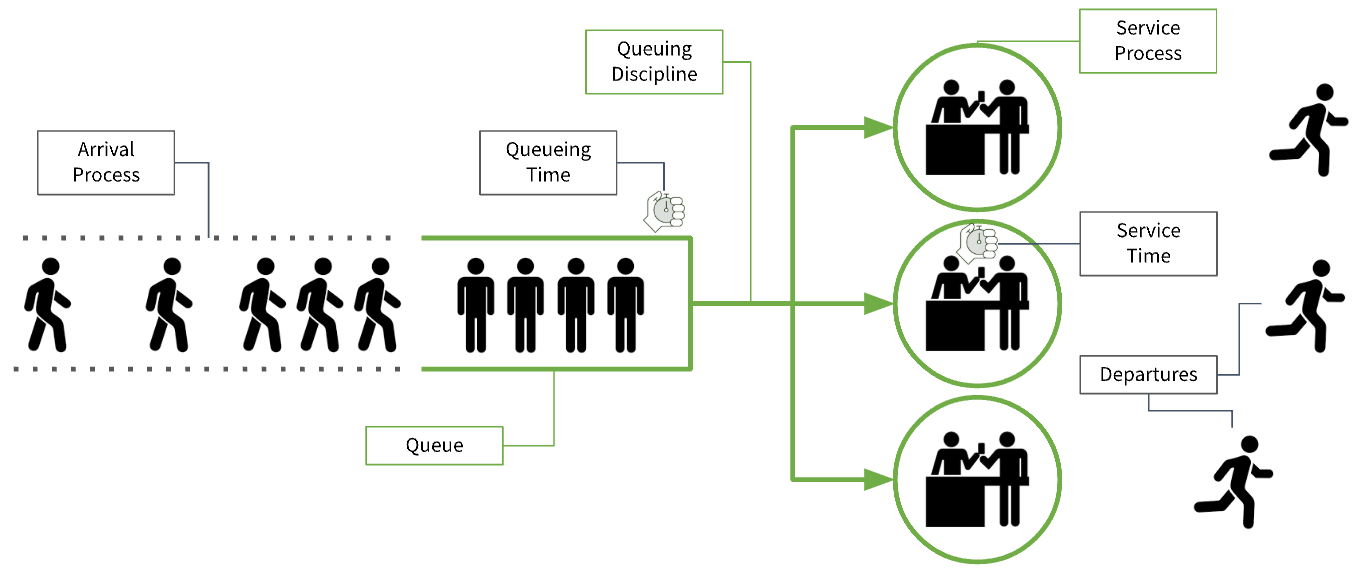
\includegraphics[width=1\linewidth]{image/queue}
\end{figure}

\subsection{ลักษณะของลูกค้า}
จำนวนผู้เข้ารับบริการ:
\begin{itemize}
	\item มีผู้เข้ารับบริการได้ไม่จำกัด
	\item มีผู้เข้ารับบริการได้จำกัด
\end{itemize}

นอกจากประเดินเรื่องความจำกัดของผู้เข้าคิวแล้ว ยังมีประเด็นเรื่องอัตราการมาเข้ารับบริการ (arrival rate) ซึ่งมักสมมติเป็น 2 รูปแบบ
\begin{itemize}
	\item ผู้เข้ารับบริการมาแบบอัตราคงที่
	\item ผู้เข้ารับบริการมาแบบสุ่ม ซึ่ง\underline{มัก}ถูกสมมติให้สุ่มด้วยการแจกแจงแบบปัวซง (Poisson distribution) 
\end{itemize}
ทั้งนี้การแจกแจงความน่าจะเป็นของการมาเข้ารับบริการอาจจะมีการแจกแจงแบบอื่นได้เช่นกันขึ้นอยู่กับสภาพแวดล้อมของแต่ละธุรกิจ

\subsubsection*{Arrival Rate: Poisson distribution}
\begin{property}
	{การแจกแจงปัวซงของอัตราการเข้ารับบริการ}{}
	กำหนดให้ $X$ เป็นตัวแปรสุ่มแทนจำนวนผู้เข้ารับบริการในช่วงระยะเวลาที่กำหนด เราจะกำหนดให้ $X$ มีการแจกแจงแบบปัวซงที่อัตราเฉลี่ยของการเข้ารับบริการมีค่าเท่ากับ $\lambda$ คนต่อหน่วยเวลา กล่าวคือ ความน่าจะเป็นที่จะมีผู้เข้าใช้บริการ $x$ คนมีค่าเท่ากับ
	$$
	P(X = x) = \frac{e^{-\lambda}\lambda^x}{x!}
	$$
\end{property}
\begin{example}
	{Warm-up Poisson}{}
	ในการทำการสำรวจอัตราการเข้าใช้บริการ ณ ร้านค้าแห่งหนึ่งในช่วงระยะเวลา 1 ชั่วโมง ผู้สำรวจพบว่าค่าเฉลี่ยการมาเข้าใช้บริการของบุคคลทั่วไปคือ 10 คน ต่อชั่วโมง กำหนดให้จำนวนผู้ใช้บริการห้างสรรพสินค้าแห่งนี้มีการแจกแจงแบบปัวซง จงหาความน่าจะเป็นต่อไปนี้
	\begin{enumerate}
		\item ความน่าจะเป็นที่จะมีผู้เข้าใช้บริการ 15 คน
		\item ความน่าจะเป็นที่จะมีผู้เข้าใช้บริการไม่เกิน 5 คน
		\item ความน่าจะเป็นที่จะมีผู้เข้าใช้บริการเกิน 5 คน
	\end{enumerate}
\end{example}
\newpage
\subsubsection*{Arrival Time Interval: Exponential distribution}
นอกจากการแจกแจงความน่าจะเป็นของจำนวนผู้เข้าใช้บริการที่มีการแจกแจงแบบปัวซงแล้วนั้น ยังมีการแจกแจงอีกแบบที่มีความสัมพันธ์เกี่ยวข้อกันคือการแจกแจงความน่าจะเป็นของระยะห่างเวลาระหว่างการเข้ามารับบริการ (arrival time interval)
\begin{property}
	{การแจกแจงเอกซ์โพเนเชียลของระยะห่างเวลาระหว่างการเข้ามารับบริการ}{}
	กำหนดให้ $X$ เป็นตัวแปรสุ่มแทนระยะห่างเวลาระหว่างการเข้ามารับบริการ เราจะกำหนดให้ $X$ มีการแจกแจงแบบเอกซ์โพเนนเชียลที่มีอัตราการเข้ามาใช้บริการเท่ากับ \(\lambda\) คนต่อหน่วยเวลา กล่าวคือ ฟังก์ชันการแจกแจงความน่าจะเป็นของตัวแปรสุ่มเวลา $T$ คือ
	\[
	f(t) = \lambda e^{-\lambda t}
	\]
	ซึ่งจะได้ว่าความน่าจะเป็นสะสม $F(a) = P(T\leq a) = 1 - e^{-\lambda a}$

\begin{center}
		\begin{tikzpicture}
		% ---- parameters you can change ----
		\def\lam{0.8} % rate \lambda > 0 (for plotting only)
		\def\a{1.5}   % left-tail cutoff 'a' (shade 0..a)
		% -----------------------------------
		
		\begin{axis}[
			width=11cm, height=7cm,
			domain=0:8, samples=400,
			axis lines=left,
			xmin=0, ymin=0, ymax=1.15*\lam,
			xlabel={$t$}, ylabel={$f(t)$},
			legend style={draw=none, fill=none},
			every axis plot/.append style={thick},
			clip=false
			]
			% pdf curve
			\addplot[name path=exp] {\lam*exp(-\lam*x)};
%			\addlegendentry{$f(t)=\lambda e^{-\lambda t}$}
			
			% baseline for fill
			\path[name path=axis0] (axis cs:0,0) -- (axis cs:\a,0);
			
			% shaded left tail 0..a
			\addplot[fill=gray!30] fill between[of=exp and axis0, soft clip={domain=0:\a}];
			
			% vertical guide at a
%			\draw[dashed] (axis cs:\a,0) -- (axis cs:\a,\lam*exp(-\lam*\a));
			\node[below] at (axis cs:\a,0) {$a$};
%			
%			% annotation of CDF on the tail
			\node[anchor=west] at (axis cs:\a,0.6*\lam)
			{$P(T\le a)=1-e^{-\lambda a}$};
		\end{axis}
	\end{tikzpicture}
\end{center}
\end{property}
\begin{example}
	{Warm-up Exponential}{}
	ในการทำการสำรวจอัตราการเข้าใช้บริการ ณ ร้านค้าแห่งหนึ่งในช่วงระยะเวลา 1 ชั่วโมง ผู้สำรวจพบว่าค่าเฉลี่ยการมาเข้าใช้บริการของบุคคลทั่วไปคือ 10 คน ต่อชั่วโมง กำหนดให้การเข้าใช้บริการเป็นกระบวนการปัวซง จงหาความน่าจะเป็นต่อไปนี้
	\begin{enumerate}
		\item ความน่าจะเป็นที่จะมีผู้เข้ามาใช้บริการภายใน 30 นาที
		\item ความน่าจะเป็นที่จะไม่มีผู้เข้ามาใช้บริการในช่วง 20 นาที
	\end{enumerate}
\end{example}

\newpage
\subsection{ลักษณะของแถวคอย}
\subsubsection{รูปแบบขอองระบบ}
\begin{enumerate}
	\item ระบบช่องทางเดียว-ขั้นตอนเดียว: ตัวอย่างเช่นตู้เอทีเอ็ม 1 ตู้
	\item ระบบช่องทางเดียว-หลายขั้นตอน: ตัวอย่างเช่นการจ่ายยาในโรงพยาบาลขนาดเล็กที่มี 1 เคาท์เตอร์จ่ายยาและ 1 เคาท์เตอร์เก็บเงินที่ผู้ป่วยจะต้องเข้าคิวจ่ายเงินก่อนแล้วค่อยเข้าคิวรับยาในขั้นตอนถัดไป
	\item ระบบหลายช่องทาง-ขั้นตอนเดียว: ตัวอย่างเช่นตู้ซื้อเหรียญโดยสาร MRT บางสถานีที่มีการเข้าคิว 1 แถวเพื่อกระจายคนไปตู้หลายตู้
	\item ระบบหลายช่องทาง-หลายขั้นตอน: ตัวอย่างเช่นแผนกจ่ายยาในโรงพยาบาลใหญ่ที่แต่ละขั้นตอนมีผู้ห้บริการมากกว่า 1 คน 
\end{enumerate}

\subsubsection{ความยาวของแถวคอย}
\begin{enumerate}
	\item จำกัด: เช่นในกรณีที่พื้นที่การเข้าแถวมีจำกัดทำให้เมื่อที่นั่งรอเต็มแล้วจะไม่สามารถรับลูกค้าเข้ามาเพิ่มได้อีกจนกว่าจะมีที่ว่าง เช่นปั๊มน้ำมัน
	\item ไม่จำกัด: เช่นเอกสารที่รอการพิมพ์ หรือระบบการจองที่ไม่ต้องอาศัยพื้นที่ทางกายภาพ
\end{enumerate}

\subsection{ลักษณะของหน่วยให้บริการ}
ในทำนองเดียวกันกับลักษณะการเข้ามาของลูกค้า เราจะสมมติให้เวลาของการให้เป็นบริการเป็นกระบวนการปัวซงเช่นกัน กล่าวคือ
\begin{itemize}
	\item การแจกแจงของเวลาให้บริการเป็นแบบเอกซ์โพเนนเชียล: กำหนดให้ $\mu$ เป็นอัตราการให้บริการโดยเฉลี่ย (คนต่อหน่วยเวลา) จะได้ว่า $f(t)=\mu e^{-\mu t}$ เมื่อ $t>0$ ซึ่งจะได้ตามมาว่า
	\(
	P(T > t) = e^{-\mu t}
	\)
	\item การแจกแจงของจำนวนคนที่ให้บริการได้ในหน่วยเวลาเป็นแบบปัวซง: กล่าวคือ \(P(X=x) = \frac{e^{-\mu}\mu^x}{x!}\)
\end{itemize}
\begin{example}
	{อัตราการ กับ เวลาที่ใช้}{}
	จงหาอัตราของการให้บริการของหน่วยบริการหนึ่งเมื่อกำหนดให้หน่วยบริการนั้นมีใช้เวลาให้บริการ 3 นาทีต่อคน
\end{example}
\newpage
\section{ตัวแบบแถวคอย (เบื้องต้น)}
ทั้งนี้ลักษณะของแถวคอยที่เราจะทำการศึกษาจะมีลักษณะดังต่อไปนี้
\begin{itemize}
	\item แถวคอยขั้นตอนเดียว
	\item หน่วยบริการมีได้ตั้งแต่ $1, 2, \dots$, หรือ $n$ หน่วยบริการ
	\item มาก่อนได้รับบริการก่อน
	\item การมารับบริการและการให้บริการเป็นแบบปัวซง (จำนวนครั้งเป็นปัวซง และระยะเวลาเป็นเอกซ์โพนเนเชียล)
\end{itemize}

\subsubsection{Kendall Notation}
เราจะเขียนรูปแบบแถวคอยเป็นสัญลักษณ์แบบ Kendall Notation ดังนี้
\begin{definition}
	{Kendall Notation}{}
	\[
	A/B/s
	\]
	โดยที่
	\begin{align*}
		A &= \text{การแจกแจงของอัตราการมารับบริการ}\\
		B &= \text{การแจกแจงของอัตราการให้บริการ}\\
		s &= \text{จำนวนหน่วยของผู้ให้บริการ}
	\end{align*}
	และสัญลักษณ์ที่ใช้แทนการแจกแจงมีดังนี้
	\begin{align*}
		M &= \text{แจกแจงแบบปัวซง}\\
		D &= \text{แจกแจงแบบคงที่}\\
		G &= \text{อัตราการให้บริการมีการแจกแจงแบบปกติ}
	\end{align*}
\end{definition}


\subsubsection{สัญลักษณ์ที่ใช้ในการวิเคราะห์แถวคอย}
\begin{definition}[breakable]
	{Notation}{}
	สัญลักษณ์ที่ใช้ในการวิเคราะห์แถวคอยมีดังนี้
	\begin{align*}
		\lambda &= \text{อัตราการเข้ามารับบริการ (จำนวนลูกค้าเฉลี่ยที่เข้ามารับบริการในหนึ่งหน่วยเวลา)}\\
		\mu &= \text{อัตราการให้บริการ (จำนวนลูกค้าเฉลี่ยที่หน่วยบริการสามารถให้บริการแล้วเสร็จในหนึ่งหน่วยเวลา)}\\
		\rho &= \text{ความน่าจะเป็นที่ระบบจะทำงาน (มีผู้รับบริการอยู่ในหน่วยบริการ)}\\
		P_0 &= \text{ความน่าจะเป็นที่ระบบจะว่าง}\\
		L &= \text{จำนวนลูกค้าโดยเฉลี่ยที่อยู่ในระบบ (ทั้งที่กำลังรับบริการและกำลังรอในแถวคอย)}\\
		L_q &= \text{จำนวนลูกค้าโดยเฉลี่ยที่อยู่ในแถวคอย}\\
		W &= \text{เวลาโดยเฉลี่ยที่ลูกค้าเสียไปในการรับบริการในระบบตั้งแต่เข้ามาจนเสร็จ}\\
		W_q &= \text{เวลาโดยเฉลี่ยที่ลูกค้าเสียไปในการรอคอยอยู่ในแถวคอย}\\
		P_n &= \text{ความน่าจะเป็นที่จะมีผู้เข้ามารับบริการจำนวน $n$ คนในระบบแถวคอย}
	\end{align*}
\end{definition}
\subsection{ตัวแบบ M/M/1}
แถวคอยที่มีอัตราการเข้ารับบริการแบบสุ่มแบบกระบวนการปัวซง, มีอัตราการให้บริการแบบปัวซอง และมี 1 หน่วยบริการ (กล่าวคือถ้ายังมี 1 คนใช้บริการอยู่คนที่เหลือต้องเข้าแถวคอยจนกว่าจะใช้บริการเสร็จและออกจากหน่วยบริการ)
\begin{theorem}
	{การวิเคราะห์เชิงปริมาณของแถวคอยแบบ M/M/1}{}
	\begin{align*}
		\rho &= \frac{\lambda}{\mu}, \qquad P_0 = 1 - \frac{\lambda}{\mu}, \qquad P_n = P_0\left(\frac{\lambda}{\mu}\right)^n \\
		L &= \frac{\lambda}{\mu - \lambda}, \qquad L_q = \frac{\lambda^2}{\mu (\mu - \lambda)} \\
		W &= \frac{1}{\mu - \lambda}, \qquad W_q = \frac{\lambda}{\mu(\mu - \lambda)}
	\end{align*}
	โดยทีสมมติฐานของตัวแบบนี้คือ $\lambda < \mu$
\end{theorem}
จริง ๆ แล้วสูตรเหล่านี้มีที่มาจากการใช้การคำนวณเชิงความน่าจะเป็น (ความน่าจะเป็น, ตัวแปรสุ่ม, การแจกแจงความน่าจะเป็นไม่ต่อเนื่อง, ค่าคาดหวัง) นักศึกษาที่แม่นในส่วนของการคำนวณเหล่านี้จะสามารถคำนวณตัวแปรต่าง ๆ ได้ด้วยตัวเองโดยที่ไม่จำเป็นต้องรู้สูตรเหล่านี้ก็ได้

%\begin{remark}
%	{ที่มาของสูตร}{}
%	กำหนดให้
%	\paragraph*{ความน่าจะเป็นที่ระบบจะทำงาน ($\rho$)} คือความน่าจะเป็นที่หน่วยบริการกำลังให้บริการผู้เข้ารับบริการอยู่ ซึ่งสามารถคำนวณหาได้โดยง่าย
%\end{remark}
\newpage
\begin{example}
	{M/M/1}{}
	บริการถ่ายเอกสารที่ร้านแห่งหนึ่งมีเครื่องถ่ายเอกสาร 1 เครื่องให้บริการแบบมาก่อนได้ก่อน โดยที่ลูกค้าที่เข้ามาเพื่อถ่ายเอกสารจะเข้ามาแบบสุ่มปัวซงในอัตรานาทีละ 2 คน ถ้าเวลาที่พนักงานประจำเครื่องถ่ายเอกสารให้บริการลูกค้ามีการแจกแจงแบบเอกซ์โพเนนเชียลด้วยค่าเฉลี่ย 1/4 นาทีต่อคน
	จงวิเคราะห์ระบบแถวคอยของบริการเครื่องถ่ายเอกสาร
\end{example}
\newpage
%\begin{example}
%	{จัดรูปสูตรให้อยู่ในรูปที่จำง่ายขึ้น}{}
%	สูตรที่ให้มาตามทฤษฎีบทเป็นสูตรที่ถูกจัดรูปให้สามารถคำนวณได้โดยใช้แค่ $\lambda$ และ $\mu$ ซึ่งอาจจะทำให้รู้สึกว่าจำได้ยาก เราจึงจะมาจัดรูปสูตรให้จำได้ง่ายขึ้นโดยใช้ความหมายเชิงปริมาณเข้ามาช่วย
%	
%	จงบอกเหตุผลว่าทำไมถึงได้สูตรดังต่อไปนี้ในเชิงความหมายเชิงปริมาณ
%	\begin{enumerate}
%		\item $P_0 = 1 - \rho$
%		\item $P_n=P_0\rho^n$
%		\item $L=\frac{\rho}{1 - \rho}$
%		\item $L_q = \rho L$
%	\end{enumerate}
%\end{example}
%\newpage
\begin{example}
	{M/M/1}{food}
	ร้านค้าแห่งหนึ่งกำลังวางแผนพัฒนาเรื่องการรอคิวของลูกค้าเพื่อไม่ให้ลูกค้าต้องรอคิวนานจึงได้ทำการวิเคราะห์พฤติกรรมลูกค้าและพบว่าจำนวนลูกค้าที่เข้ามาซื้อสินค้าโดยเฉลี่ยจะอยู่ที่ 20 คนต่อชั่วโมงและมีการแจกแจงแบบปัวซอง ในส่วนของทางร้าน พนักงานของร้านสามารถให้บริการคิดชำระเงินได้เฉลี่ย 1 คนต่อ 2 นาทีและมีการแจกแจงของเวลาการให้บริการแบบเอ็กซ์โพเนนเชียล ปัจจุบันทางร้านมีพนักงาน 1 คน จงวิเคราะห์แถวคอยของร้านค้าแห่งนี้ 
\end{example}
\newpage

\subsection{ตัวแบบ M/M/s}
\begin{theorem}
	{การวิเคราะห์เชิงปริมาณของแถวคอยแบบ M/M/s}{}
	\begin{align*}
		\rho &= \frac{\lambda}{s\mu}, \qquad 
		P_0 = \frac{1}{\sum_{n=0}^{s-1} \frac{(\lambda/\mu)^n}{n!} + \left[ \frac{(\lambda/\mu)^s}{s!} \frac{s\mu}{s\mu - \lambda} \right]}\\
		P_n &= \begin{cases}
			P_0\frac{(\lambda/\mu)^n}{n!} &\text{เมื่อ\quad} n\leq s\\
			P_0\frac{(\lambda/\mu)^n}{s!s^{n-s}} &\text{เมื่อ\quad} n > s
		\end{cases}\\
		L_q &= P_0\left[\frac{(\lambda/\mu)^s \rho}{s!(1-\rho)^2}\right], \qquad L = L_q + \frac{\lambda}{\mu}\\
		W_q &= \frac{L_q}{\lambda}, \qquad W = W_q + \frac{1}{\mu}
	\end{align*}
	โดยทีสมมติฐานของตัวแบบนี้คือ $\lambda < s\mu$
\end{theorem}
\begin{example}
	{M/M/s}{}
	บริการถ่ายเอกสารที่ร้านแห่งหนึ่งมีเครื่องถ่ายเอกสาร 5 เครื่องให้บริการแบบมาก่อนได้ก่อน โดยที่ลูกค้าที่เข้ามาเพื่อถ่ายเอกสารจะเข้ามาแบบสุ่มปัวซงในอัตรานาทีละ 2 คน ถ้าเวลาที่พนักงานประจำเครื่องถ่ายเอกสารให้บริการลูกค้ามีการแจกแจงแบบเอกซ์โพเนนเชียลด้วยค่าเฉลี่ย 1/4 นาทีต่อคน
	จงวิเคราะห์ระบบแถวคอยของบริการเครื่องถ่ายเอกสาร
\end{example}
\newpage

\subsection{ตัวแบบ M/G/1}
(ข้ามสำหรับ 720201)
\subsection{ตัวแบบ M/D/1}
(ข้ามสำหรับ 720201)
\section{ตัวแบบแถวคอย (ทฤษฎี)}
(ข้ามสำหรับ 720201)

\section{การวิเคราะห์ระบบแถวคอยเพื่อการตัดสินใจทางธุรกิจ}
ชัดเจนว่าวิธีการหนึ่งที่จะทำให้ลูกค้าไม่ต้องรอคอยคือการเพิ่มหน่วยบริการเข้าไปให้มากพอ หรือมากกว่าลูกค้าที่เข้ามา ก็จะทำให้ลูกค้าทุกคนสามารถได้รับบริการได้ทันที ทว่าวิธีการดังกล่าวอาจจะเป็นไปไม่ได้เพราะใช้ต้นทุนสูงหรือทรัพยากรไม่เพียงพอ (เช่นพื้นที่ร้าน) เราจึงต้องทำการ trade-off กันระหว่างจำนวนหน่วยบริการกับต้นทุนที่ใช้

ทั้งนี้ ต้นทุนที่จะนำมาพิจารณาในการวิเคราะห์แถวคอยมี 2 หมวดดังนี้
\begin{enumerate}
	\item \textbf{ต้นทุนการให้บริการ} (service cost): เช่นค่าแรงงาน ค่าเช่าสถานที่ ที่แปรผันตรงกับจำนวนหน่วยบริการ กล่าวคือ ยิ่งเพิ่มหน่วยบริการมากขึ้น ก็จะใช้ต้นทุนมากขึ้นเรื่อย ๆ
	\item \textbf{ต้นทุนในการรอคอยของลูกค้า} (waiting cost): เป็นค่าเสียหายที่เกิดจากการรอคอยที่ยิ่งลูกค้ารอคอยนานเท่าไหร่ก็จะยิ่งมีค่าใช้จ่ายมากขึ้นเท่านั้น เช่นการประเมิณความพึงพอใจของลูกค้า หรือต้นทุนของบริการเพิ่มเติมที่ลูกค้าได้รับขณะรอคิว (เช่นร้าน Haidilao มีบริการทำเล็บหรือขนมฟรีของลูกค้าที่กำลังรอคิว)
\end{enumerate}
\begin{align*}
	\text{ค่าใช้จ่ายรวม} &= \text{ต้นทุนการให้บริการ} + \text{ต้นทุนการรอคอยของลูกค้า}\\
				TC &= s\cdot C_s + L\cdot C_w 
\end{align*}

\begin{tikzpicture}
	\begin{axis}[
%		axis lines=middle,
		xmin=-0.5, xmax=5,
		ymin=-0.5, ymax=6,
		samples=200,
		domain=0.01:5,   % to avoid x=0 singularity
		legend style={at={(1,1)},anchor=north east},
		xlabel={\textbf{จำนวนหน่วยบริการ}},
		ylabel={\textbf{ค่าใช้จ่าย}}
		]
		
		% (1) y = 1/x
		\addplot[blue, thick] {1/x};
%		\addlegendentry{$y = \tfrac{1}{x}$}
		
		% (2) y = x
		\addplot[red, thick] {x};
%		\addlegendentry{$y = x$}
		
		% (3) y = x + 1/x
		\addplot[green!60!black, thick, dashed] {x + 1/x};
%		\addlegendentry{$y = x + \tfrac{1}{x}$}
		
	\end{axis}
\end{tikzpicture}
\subsection{การกำหนดจำนวนหน่วยบริการ}
โจทย์ที่มักจะถูกถามเป็นอันดับแรกคือเราควรจะทำหน่วยบริการกี่หน่วยดีเพื่อให้เพียงพอที่จะทำให้ลูกค้าพอใจโดยที่ไม่ต้องใช้ต้นทุนเยอะจนเกินไป ซึ่งวิธีการคือการวิเคราะห์หาจุดต่ำสุดของค่าใช้จ่ายรวม
แต่ในทางปฏิบัติ เนื่องจากเราต้องการหาจุดเหมาะสุดของตัวแปรเดียวที่เป็นจำนวนนับ จึงเป็นการง่ายที่จะทำการวิเคราะห์หาต้นทุนรวมของ M/M/1, M/M/2, ... ไปเรื่อย ๆ จนเจอจุดที่ให้ค่าต่ำสุด (ลดลงเรื่อย ๆ จนเจอจุดที่เพิ่มอีกหน่วยแล้วมีต้นทุนมากขึ้น)
\begin{example}
	{}{food2}
	จากตัวอย่าง \ref{ex:food} ที่จำนวนลูกค้าที่เข้ามาซื้อสินค้าโดยเฉลี่ยจะอยู่ที่ 20 คนต่อชั่วโมงและมีการแจกแจงแบบปัวซอง, พนักงานของร้านสามารถให้บริการคิดชำระเงินได้เฉลี่ย 1 คนต่อ 2 นาทีและมีการแจกแจงของเวลาการให้บริการแบบเอ็กซ์โพเนนเชียล สมมติว่าปัจจุบันมีพนักงาน 3 คนอยู่แล้ว จงหาว่าร้านนี้ควรจ้างพนักงานบริการชำระเงินเพิ่มอีกกี่คนมาทำงาน
\end{example}
\newpage

\subsection{การตัดสินใจจัดรูปแบบแถวคอย}
\begin{example}
	{}{}
	จากตัวอย่าง \ref{ex:food2} มีนักวิเคราะห์เสนอว่าแทนที่จะเพิ่มจำนวนพนักงานให้ลองเปลี่ยนรูปแบบเป็นแต่ละพนักงานมีแถวคอยเป็นของตัวเอง และลูกค้าที่เข้ามาจะกระจายตัวกันตามแถวคอยทั้ง 3 แถว กล่าวคือลองเปลี่ยนจาก M/M/3 เป็น M/M/1 ทั้งหมด 3 ระบบอิสระจากกัน จงวิเคราะห์ต้นทุนรวมของระบบใหม่นี้
\end{example}
\newpage

\subsection{การตัดสินใจในลักษณะอื่น ๆ}
\begin{example}
	{}{}
	บริษัทโลจิสติกแห่งหนึ่งให้บริการทั่วไปเกี่ยวกับการขนส่งและจัดเก็บสินค้า โดยปัจจุบันมีโกดังเก็บสินค้าเพียงแห่งเดียว ซึ่งมีที่เทียบรถบรรทุกเพื่อขนส่งสินค้าขึ้นลงได้ครั้งละ 1 คัน รถเข้ามาเฉลี่ยทุก ๆ 40 นาที แจกแจงแบบเอ็กซโพเนนเชียล การขนสินค้าขึ้นลงใช้เวลาเฉลี่ยคันละ 30 นาที แจกแจงแบบเอ็กซโพเนนเชียล ถ้าบริษัทต้องการให้รถแต่ละคันใช้เวลาในระบบการขนถ่ายสินค้าไม่เกินคันละ 1 ชั่วโมง ควรใช้เวลาในการขนสินค้าคันละกี่นาที
\end{example}
\newpage


%\section{การวิเคราะห์แถวคอยโดยกระบวนการมาร์คอฟ}